\documentclass[a4paper,10pt]{article}
\usepackage[utf8]{inputenc}
\usepackage{amssymb}
\usepackage{graphicx}
\usepackage{hyperref}
\usepackage{algorithm,algpseudocode}
\usepackage{default}
\usepackage{tikz}
\usepackage{xcolor}
\usepackage[francais]{babel}
\usepackage[top=3cm,bottom=3cm,right=3cm,left=3cm]{geometry}

\begin{document}

\author{LIMBALLE Pierre - PEREZ Quentin}
\title{Méthodes et Outils pour la Programmation\\% 
Mini Projet 2015}
\definecolor{primary}{RGB}{37,72,124}
\definecolor{secondary}{RGB}{253,250,200}

    
%\addtobeamertemplate{footline}{\insertframenumber/\inserttotalframenumber\\}
 %\addtobeamertemplate{sidebar bottom}{\insertframenumber}
\makeatletter
  \begin{titlepage}
  \centering
      {\LARGE \textbf{LIMBALLE Pierre - PEREZ Quentin}}\\
      UFR-ST - Licence informatique 3ème année\\Groupe TP 2B\\
    \vspace{2cm}
      {\LARGE \@date\\}
    \vspace{1cm}
        
\includegraphics[width=0.3\textwidth]{java.png}\\
    \vspace{1em}
       {\LARGE \textbf{\@title}\\
    \vspace{1em}
       Rapport\\} 
    \vspace{2em}
    \vspace{1cm}
        
\includegraphics[width=0.7\textwidth]{ufrst.jpg}\\
    \vspace{1.5cm}
      {Contacts : \href{mailto:pierre.limballe@edu.univ-fcomte.fr}{pierre.limballe@edu.univ-fcomte.fr}, \href{mailto:quentin.perez@edu.univ-fcomte.fr}{quentin.perez@edu.univ-fcomte.fr}\\Professeurs : GREFFIER Françoise, BONNEVILLE François}
    \vfill
        %\includegraphics[width=0.7\textwidth]{radare.png}\\
  \end{titlepage}
\makeatother

\newpage
\tableofcontents
\newpage

\section{Sujet}
\subsection{Contexte}
Dans le cadre du module de Méthodes et Outils pour la Programmation (MOP), la réalisation d'un projet nous a été demandé afin de mettre
en application les connaissances théoriques acquisent tout au long du semestre 5. \\
La conception de l'application a pour objectifs :
\begin{itemize}
  \item l'utilisation du langage de programmation Java en Orienté Objet
  \item l'application du paradigme MVC (Modèle - Vue - Contrôleur)
  \item l'approche du travail collaboratif par l'utilisation de logiciels de gestion de versions
  \item la manipulation d'éléments graphiques de la bibliothèque graphique JavaSwing
\end{itemize}

\subsection{But de l'application}
La finalité de ce projet est la conception d'une application Java qui réalise une animation graphique en 2D, 
représentant un ensemble de planètes et leurs satellites en orbite autour d'une ou plusieurs étoiles.
L'utilisateur doit disposer des fonctionnalités suivantes :
\begin{itemize}
  \item l'ajout et la suppression d'astres (étoiles ou satellites) dans l'application
  \item l'affichage des astres dans une fenetre graphique animée
  \item la possibilité de sauvegarder un système planétaire 
\end{itemize}
La contrainte d'ergonomie est également importante quant à l'utilisation du logiciel.

\newpage
\section{Conception}
\subsection{Introduction}
Planethacks est le nom choisi pour l'application. Du fait d'un travail en binôme, l'utilisation
d'un logiciel de gestion de version fut priviligiée. Nous avons pour cela utilisé Git, en lien avec le serveur d'hébergement \href{https://github.com}{GitHub} (sources GitHub de Planethacks : \url{https://github.com/qperez/planetacks}). 
\begin{center}
  $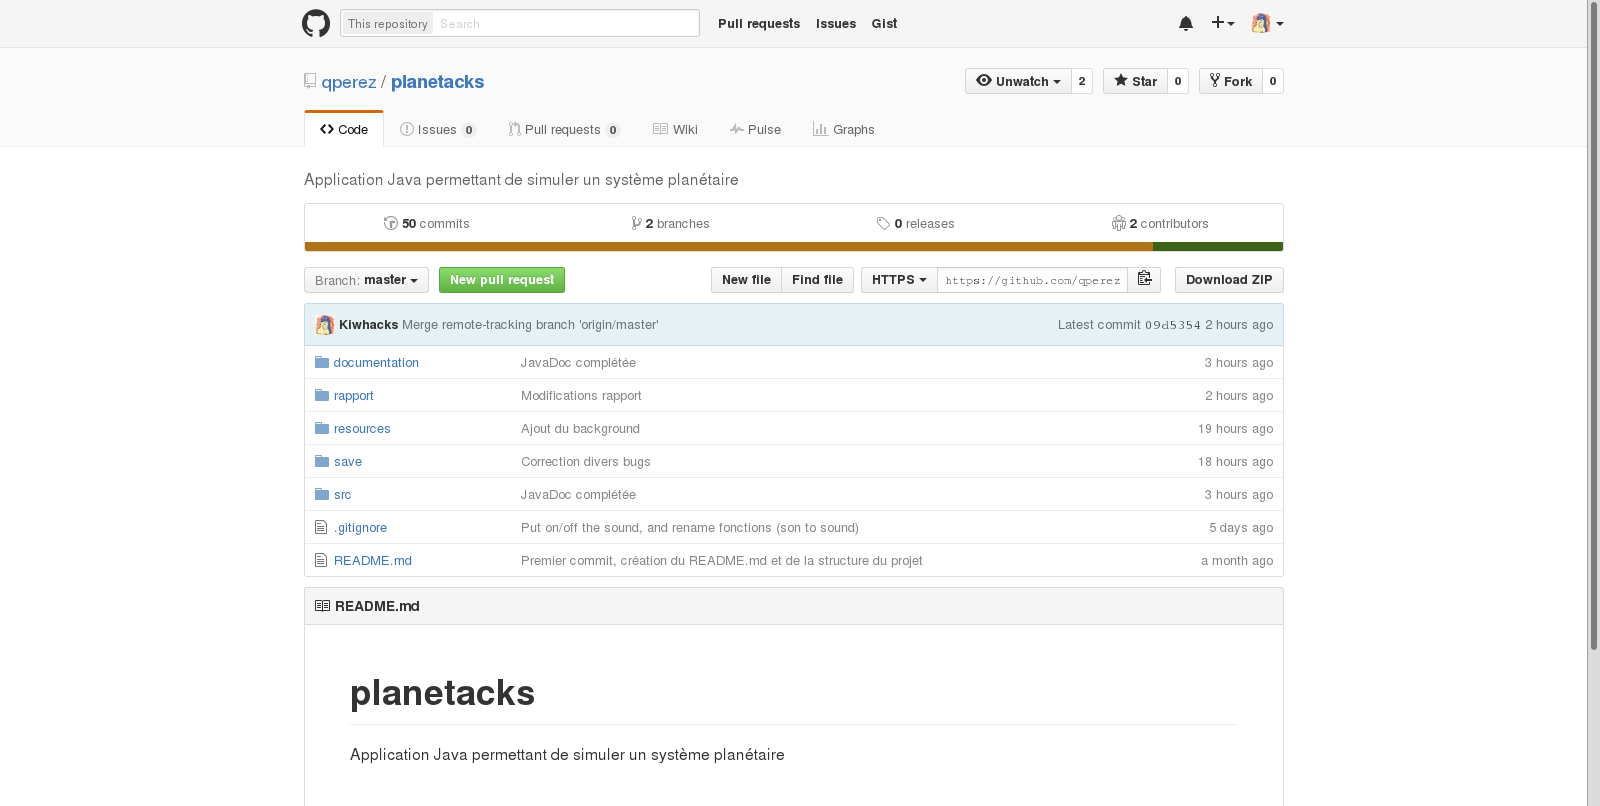
\includegraphics[scale=0.3]{git.png}$
\end{center}


L'IDE (\textit{Internal Development Environement}) IntelliJ IDEA fut utilisé durant toute la phase de développement et de tests, et ce afin 
d'accélérer et de faciliter le développement de l'application ainsi que son déboguage.\\
\begin{center}
  $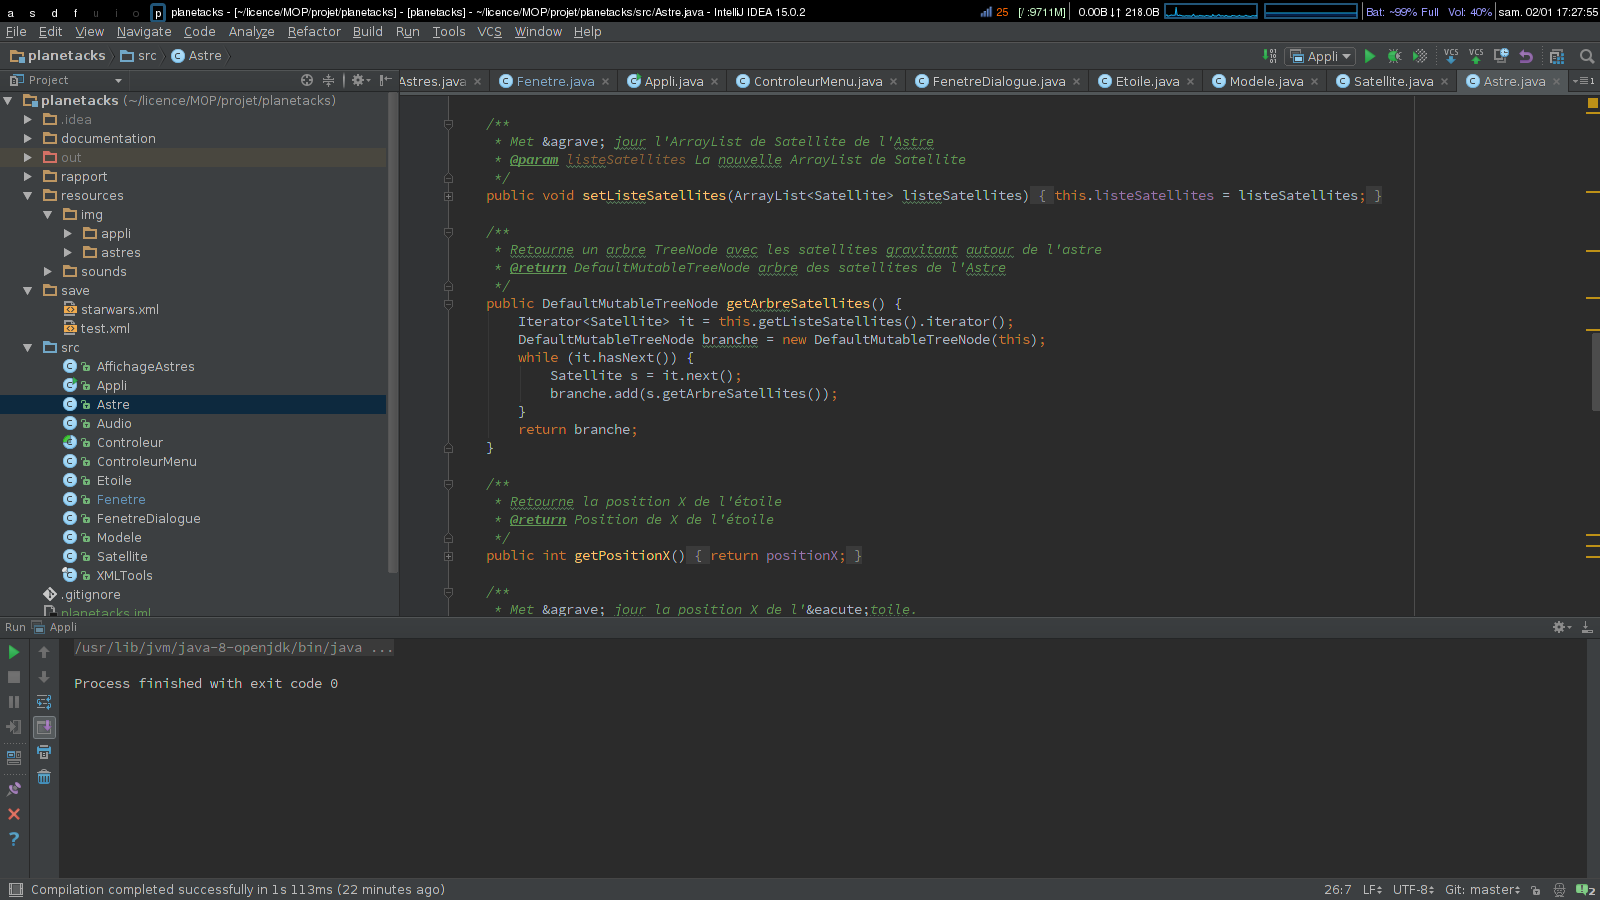
\includegraphics[scale=0.3]{idea.png}$
\end{center}

\newpage
\subsection{Structures de données au sein de l'application}
La définition de classes permettant de structurer les données de notre programme fut la première étape de conception. Ainsi 3 classes 
nous permettent de modéliser un astre :
\begin{itemize}
  \item Astre (classe abstraite)
  \item Etoile
  \item Satellite
\end{itemize}

Planethacks repose sur une conception basée sur le paradigme MVC. Ce paradigme impose l'utilisation à minima de 3 classes (Modèle - Vue - Contrôleur) permettant de
séparer les données de l'affichage et des interactions utilisateur. \\ 
Dans un soucis de respect du modèle MVC, nous disposons donc des classes suivantes :
\begin{itemize}
  \item Fenetre
  \item Modele
  \item Controleur (classe abstraite)
  \item ControleurMenu
  \item AffichageAstres
\end{itemize}

Afin de réaliser la fonctionnalité de sauvegarde, une classe spécifique contenant les outils nécessaires fut créée : \textit{XMLTools}. \\
Le point d'entrée de l'application est assurée par la classe \textit{Appli}.

\subsubsection{Modélisation d'un astre (Etoile ou Satellite)}
Le diagramme UML ci-dessous représente la modélisation choisie pour un astre :
\begin{center}
  $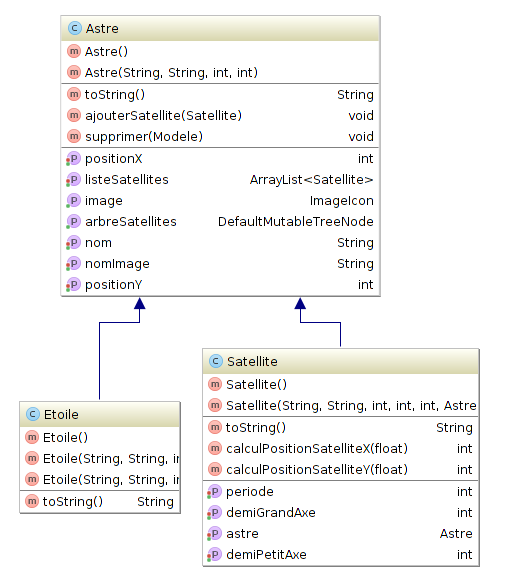
\includegraphics[scale=0.4]{classes_astre.png}$
\end{center}
Les méthodes \textit{calculPositionSatelliteX(float)} et \textit{calculPositionSatelliteX(float)} présentes dans la classe Satellite permettent
de calculer la position en X et en Y du Satellite en fonction du temps. La méthode \textit{ajouterSatellite(Satellite)} permet de mettre en orbite un satellite autour d'un astre. Enfin, la méthode \textit{supprimer(Modele)} permet de supprimer récursivement un astre et ses satellites à partir du modèle donné.

\newpage
\subsection{Structure générale de l'application}
\subsubsection{Emplacement des fichiers}
Nous avons utilisé une structure de fichiers qui nous parraissait être la plus simple et la meilleure pour le fonctionnement de l'application. Ci-dessous, une représentation de l'arborescence :\\
\begin{center}
  $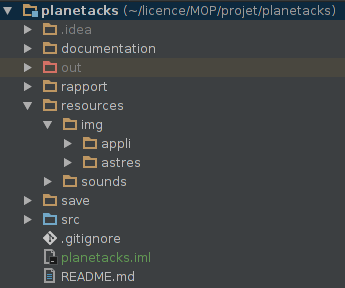
\includegraphics[scale=0.7]{arbo.png}$
\end{center}

Nous pouvons retrouver les dossiers de production suivants, dans lesquels nous manipulions directement les fichiers :
\begin{itemize}
 \item \begin{verbatim}src\end{verbatim} $\rightarrow$ dossier des sources (.java)
 \item \begin{verbatim}ressources\end{verbatim} $\rightarrow$ dossier des différents fichiers image ou audio
 \begin{itemize}
  \item \begin{verbatim}img\end{verbatim} $\rightarrow$ dossier contenant toutes les images du projet
  \begin{itemize}
   \item \begin{verbatim}appli\end{verbatim} $\rightarrow$ dossier des images de l'application en général
   \item \begin{verbatim}astres\end{verbatim} $\rightarrow$ dossier des images des astres (.png)
  \end{itemize}
  \item \begin{verbatim}sounds\end{verbatim} $\rightarrow$ dossier contenant tous les sons du projet
 \end{itemize}
 \item \begin{verbatim}rapport\end{verbatim} $\rightarrow$ dossier contenant les fichiers permettant de réaliser ce rapport (fichiers \LaTeX)
\end{itemize}
\vspace{0.5cm}
Mais également des dossiers dont le contenu est généré automatiquement :
\begin{itemize}
 \item \begin{verbatim}out\end{verbatim} $\rightarrow$ dossier des fichiers java compilés (.class)
 \item \begin{verbatim}save\end{verbatim} $\rightarrow$ dossier des fichiers de sauvegarde générés par l'application (.xml)
 \item \begin{verbatim}documentation\end{verbatim} $\rightarrow$ dossier contenant la documentation du projet (.html)
 \item \begin{verbatim}.idea\end{verbatim} $\rightarrow$ dossier contenant les fichiers de configuration du logiciel \textit{IntelliJ IDEA}
\end{itemize}
\vspace{0.5cm}
Ainsi que des fichiers seuls :
\begin{itemize}
 \item \begin{verbatim}.gitignore\end{verbatim} $\rightarrow$ fichier permettant d'ignorer l'envoi de fichiers sur GitHub (ex : dossier \textit{out})
 \item \begin{verbatim}README.md\end{verbatim} $\rightarrow$ fichier MarkDown de présentation du projet sur GitHub
 \item \begin{verbatim}planetacks.iml\end{verbatim} $\rightarrow$ fichier de configuration du projet pour \textit{IntelliJ IDEA}
\end{itemize}

\subsubsection{Architecture MVC}
\begin{center}
  $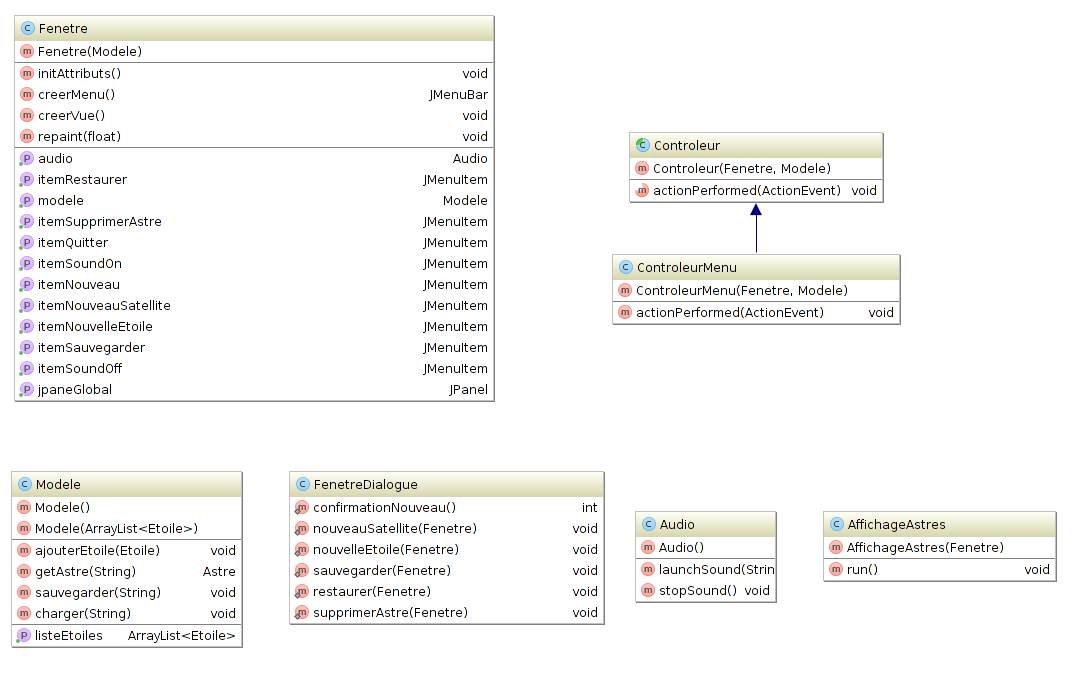
\includegraphics[scale=0.4]{classes_mvc.png}$
\end{center}

Comme dit précédemment, nous avons utilisé le paradigme MVC afin de faciliter le développement. Dans cette architecture, nous pouvons retrouver 3 principales classes qui sont les représentantes du modèle MVC : 
\begin{itemize}
 \item \textit{Modele} abstraite implémentant la classe \textit{ActionListener}
 \item \textit{Fenetre} étendue de la classe \textit{JFrame}
 \item \textit{Controleur}
\end{itemize}

La classe \textit{Modele} nous permet de gérer la liste des astres, comme par exemple ajouter une Etoile, ainsi que l'enregistrement et la restauration d'un système planétaire. Plus généralement, elle est le modèle des données de l'application.

La class \textit{Fenetre} s'occupe de tout ce qui touche à l'interface utilisateur, sauf la gestion des différents pop-up que nous verrons dans la classe \textit{FenetreDialogue}. Elle regroupe la présentation et le design de l'application, comme le menu, l'image de fond...

La classe \textit{Controleur} quant à elle, permet de faire le lien entre les deux classes précédente. Elle permet donc la gestion des événements, ainsi que la synchronisation entre les données et l'affichage.

Ici, le contrôleur connait la vue et le modèle, la vue ne connait que le modèle, tandis que le modèle n'a pas d'informations sur les deux autres.\\

La classe \textit{ControleurMenu} ne contrôle uniquement le menu et les actions qu'il peut avoir. Elle est étendue de la classe \textit{Controleur}.

La classe \textit{FenetreDialogue} prend en compte toutes les interactions avec l'utilisateur, comme l'ajout d'un astre, ou encore la sauvegarde d'un système planétaire.

La classe \textit{AffichageAstres} étendue de la classe \textit{Thread}, permet de lancer une boucle infinie pour desssiner les astres sur la fenêtre principale.

La classe \textit{Audio} nous permet de gérer plus facilement la lancement et l'arrêt du son de l'application.

\newpage
\subsection{Les algorithmes intéressants}

\begin{algorithm}
\caption{méthode repaint de la classe Fenetre}
\begin{algorithmic}
\Function{repaint}{t temps}
\State Supprimer l'ensemble des composants graphique du JPanel
\For{chaque Etoile $e$ de la liste d'étoiles du Modele}
    \State $jlabastre\gets$ nouveau JLabel avec l'image de $e$
    \State Afficher $jlabastre$ en fonction de la position $X_{e}$ et $Y_{e}$
    \State Ajouter le $jlabastre$ au JPanel
    \State Appel de la fonction $repaintSatellite$ avec $e.getListeSatellite()$ et $t$
\EndFor
\State Appel de la méthode $repaint()$ sur le JPanel
\EndFunction
\end{algorithmic}

\begin{algorithmic}
\Function{repaintSatellite}{listeSatellite $l$, temps $t$}
\For{chaque Satellite $s$ de la liste des satellites $l$}
  \State $jlabsat\gets$ nouveau JLabel avec l'image de $s$
  \State Afficher $jlabsat$ en fonction de $s.calculPositionSatelliteX(t)$ et $s.calculPositionSatelliteY(t)$
  \State Ajouter le $jlabsat$ au JPanel
  \State Appel récursif de $repaintSatellite$
\EndFor
\EndFunction
\end{algorithmic}
\end{algorithm}

\begin{algorithm}
\caption{méthode encodeFromFile de la classe XMLTools}
 \begin{algorithmic}
\Function{decodeFromFile}{Object $object$, String $fileName$}
\State $fos\gets$ nouveau FileOutputStream initialisé avec $fileName$
\State $decoder\gets$ nouveau XMLEncoder initialisé avec $fos$
\State écrire $object$ dans le buffer I/O avec $encoder.writeObject(object)$
\State flush du buffer I/O avec $encoder.flush()$
\EndFunction
 \end{algorithmic}
\end{algorithm}

\begin{algorithm}
\caption{méthode decodeFromFile de la classe XMLTools}
 \begin{algorithmic}
\Function{decodeFromFile}{Object $object$, String $fileName$}
\State $fis\gets$ nouveau FileInputStream initialisé avec $fileName$
\State $decoder\gets$ nouveau XMLEncoder initialisé avec $fis$
\State $object\gets$ l'objet renvoyé par $decoder.readObject()$
\State $la\gets$ transtypage de $object$ en ArrayList d'Astre
\State $it\gets$ nouvelle itérateur d'ArrayList d'Astre
\While{$it$ retourne qu'il reste un élément à parcourir}
  \State $astre\gets$ élément suivant Astre pointé par $it$
  \State mise à jour de l'image de l'image de $astre$ à l'aide de $a.setImage()$
\EndWhile \\
\Return $la$
\EndFunction
 \end{algorithmic}
\end{algorithm}

\newpage
\subsection{Points intéressants et supplémentaires du programme}
Afin d'être original, avons décidé de créer un "mode" \textit{StarWars}. 

Tout d'abord, il a fallu recréer des nouvelles planètes tirées de la saga, comme \textit{Tatooine}, \textit{Naboo}, \textit{Jakku}, l'\textit{étoile noire} ainsi qu'un \textit{fighter} (vaisseau côté obscur de la force) ou encore le \textit{Faucon Millenium} d'Han Solo. Ceci nous a fait découvrir l'utilisation de zones transparentes dans une image PNG, ainsi que le logiciel Gimp que nous n'avions pas utilisé dans notre formation jusqu'à présent.

De plus, nous avons implémenté la gestion du son, que l'on peut activer ou désactiver grâce à un menu prévu à cet effet. Celui-ci s'active automatiquement lorsque l'on charge la sauvegarde de l'environnement \textit{StarWars}, avec le thème original des 7 films accompagné de plusieurs bruitages célèbres. L'intégration de son dans une application était inconnue pour nous auparavant, c'est pourquoi nous avons décidé de l'ajouter à notre projet pour la découvrir.

\subsection{Tests}
Les tests ainsi que la documentation ont été réalisés tout au long du développement. Ceci nous a permis de pouvoir déboguer facilement et de ne pas perdre de temps dans la production à cause d'erreurs de programmation. Les outils utilisés pour la construction du projet nous ont aussi facilité les tests. 

En effet, \textit{IntelliJ IDEA} propose des fonctionnalités permettant d'éviter un grand nombre d'erreurs (auto-complétion inter-classes, renommage des variables et fonctions sur tout le projet, messages explicites lors d'une erreur...) et de passer moins de temps sur des problèmes de syntaxe. 

De plus, grâce au gestionnaire de version GitHub, il est aisé de retrouver les modifications apportées à un fichier, et pourquoi elles ont été faites. Ici encore, cela permet de gagner du temps et de pouvoir retrouver un projet fonctionnel même après avoir rencontré un problème lourd lors du développement. 

Pour finir, ces deux logiciels fonctionnent l'un avec l'autre, ce qui rend la construction du projet très confortable.
\\

Une phase de tests fonctionnels plus conséquente a été réalisée à la fin du projet. Dans un souçis de professionnalisation et de rigueur quant à
la démarche de tests, plusieurs fiches de vérification d'aptitude au bon fonctionnement de l'application ont été réalisées.
\\

Pour ce qui est des tests des entrées utilisateur lors du déroulement du programme, nous testons si le type des données rentrées est bon. Par exemple, si nous attendons un entier et que l'utilisateur rentre ``toto'', un message est affiché à l'écran. De même, si l'utilisateur a oublié de remplir un champ, il lui sera annoncé à l'écran et il ne pourra pas valider son ajout ou sa suppression d'astre tant que les données ne sont pas conformes.

\newpage
\begin{tikzpicture}[remember picture,overlay]
	\draw[very thick]
		([yshift=-15pt,xshift=15pt]current page.north west)--
		([yshift=-15pt,xshift=-15pt]current page.north east)--
		([yshift=15pt,xshift=-15pt]current page.south east)--
		([yshift=15pt,xshift=15pt]current page.south west)--cycle;


\end{tikzpicture}
\begin{center}
  \begin{huge}
    Vérification d'aptitude au bon fonctionnement \\
  \end{huge}
  \vspace{1cm}
  \begin{Large}
    Scénario de test numéro 1
  \end{Large}
\end{center}
\rule{\linewidth}{.5pt}
Profil d'utilisateur visé: Étudiant \\\\
Titre du scénario: Création et sauvegarde d'un système planétaire \\\\
Conditions préalables:
\begin{itemize}
 \item Disposer d'un ordinateur ayant Java Runtime Environement installé
 \item Disposer du logiciel Planethacks
 \item Aucunes aides à la prise en main ou à la décision durant la durée du test
\end{itemize}
Description: on souhaite vérifier que l'application permet l'ajout de 2 étoiles ainsi que de 3 satellites. 
On désire ensuite sauvegarder l'ensemble du système planétaire créé dans un fichier ``test.xml''.
Le test s'effectue sans jeu de données préalables.
\begin{center}
 \begin{Large}
    Instructions du scénario
  \end{Large}
\end{center}
\begin{enumerate}
 \item Ne pas ouvrir de nouveau système planétaire à l'ouverture de l'application
 \item Ajouter une étoile se nommant Tatooine en position X=250 et Y=300 et ayant pour image ``tatooine.png''
 \item Ajouter un satellite à l'étoile Tatooine se nommant Asteroide et ayant un demi-grand axe=50, un demi-petit axe = 50, une période 
 de 150 et ayant pour image ``asteroide.png'' 
 \item Ajouter un satellite à l'étoile Tatooine se nommant Faucon et ayant un demi-grand axe=50, un demi-petit axe = 50, une période 
de 150 et ayant pour image ``faucon\_millenium.png''
 \item Ajouter une étoile se nommant Terre en position X=600 et Y=400 et ayant pour image ``terre.png''
 \item Ajouter un satellite à l'étoile Terre se nommant Lune et ayant un demi-grand axe=200, un demi-petit axe=50, une période 
 de 80 et ayant pour image ``lune.png''
 \item Sauvegarder le système planétaire sous le nom ``test''
 \item Quitter l'application
 \item Vérifier que test.xml a été créé
\end{enumerate}

\newpage
\begin{tikzpicture}[remember picture,overlay]
	\draw[very thick]
		([yshift=-15pt,xshift=15pt]current page.north west)--
		([yshift=-15pt,xshift=-15pt]current page.north east)--
		([yshift=15pt,xshift=-15pt]current page.south east)--
		([yshift=15pt,xshift=15pt]current page.south west)--cycle;
\end{tikzpicture}

\begin{center}
  \begin{huge}
    Vérification d'aptitude au bon fonctionnement \\
  \end{huge}
  \vspace{1cm}
  \begin{Large}
    Scénario de test numéro 2
  \end{Large}
\end{center}
\rule{\linewidth}{.5pt}
Profil d'utilisateur visé: Étudiant \\\\
Titre du scénario: Chargement et modification d'un système planétaire \\\\
Conditions préalables:
\begin{itemize}
 \item Disposer d'un ordinateur ayant Java Runtime Environement installé
 \item Disposer du logiciel Planethacks
 \item Disposer d'un jeu de données correpondant à une sauvegarde d'un système planétaire
 \item Aucunes aides à la prise en main ou à la décision durant la durée du test
\end{itemize}
Description: on souhaite vérifier que l'application puisse charger correctement un système planétaire enregistré au format 
XML mais également qu'il puisse être modifié, c'est à dire que 2 astres puissent être supprimés et un autre ajouté. 
Le test s'effectue avec jeu de données ``starwars.xml''.
\begin{center}
 \begin{Large}
    Instructions du scénario
  \end{Large}
\end{center}
\begin{enumerate}
 \item Choisir d'ouvrir un nouveau système planétaire lors du démarrage de l'application, choisir ``starwars.xml''
 \item Supprimer l'astre ``tatooine''
 \item Ajouter une étoile se nommant Terre en position X=600 et Y=400 et ayant pour image ``terre.png''
 \item Supprimer l'astre ``etoile noire''
 \item Quitter l'application
\end{enumerate}

\newpage
\begin{tikzpicture}[remember picture,overlay]
	\draw[very thick]
		([yshift=-15pt,xshift=15pt]current page.north west)--
		([yshift=-15pt,xshift=-15pt]current page.north east)--
		([yshift=15pt,xshift=-15pt]current page.south east)--
		([yshift=15pt,xshift=15pt]current page.south west)--cycle;
\end{tikzpicture}

\begin{center}
  \begin{huge}
    Vérification d'aptitude au bon fonctionnement \\
  \end{huge}
  \vspace{1cm}
  \begin{Large}
    Scénario de test numéro 3
  \end{Large}
\end{center}
\rule{\linewidth}{.5pt}
Profil d'utilisateur visé: Étudiant \\\\
Titre du scénario: Vérification de l'activation de la désactivation de l'environnement sonore et de la fonction de fermeture de l'application \\\\
Conditions préalables:
\begin{itemize}
 \item Disposer d'un ordinateur ayant Java Runtime Environement installé
 \item Disposer du logiciel Planethacks
 \item Disposer d'enceintes stéréo (le surround est en option dans certaines salles équipées) 
 \item Aucunes aides à la prise en main ou à la décision durant la durée du test
\end{itemize}
Description: on souhaite vérifier que l'on puisse activer ou désactiver l'environnement sonore de l'application mais également
que la fonction permettant de quitter l'application fonctionne correctement.
Le test s'effectue sans jeu de données préalables.
\begin{center}
 \begin{Large}
    Instructions du scénario
  \end{Large}
\end{center}
\begin{enumerate}
 \item Ne pas ouvrir de nouveau système planétaire à l'ouverture de l'application
 \item Activer le son et vérifier que le thème original de Star Wars est entendu
 \item Désactiver le son
 \item Activer le son et vérifier que le thème original de Star Wars est entendu
 \item Quitter l'application à l'aide du menu
\end{enumerate}

\newpage
\newpage
\section{Conclusion}
\subsection{Bilan}
Nous avons pu répondre aux différents points demandés à savoir :
\begin{itemize}
 \item Créer un astre qui est ajouté dynamiquement à l'ensemble des astres de l'appli
 \item Supprimer un astre dynamiquement de l'application
 \item Enregistrer sur le disque un fichier comprenant une étoile et ses satellites
 \item Ouvrir un fichier enregistré comprenant une étoile et ses satellites
 \item JavaDoc générée du programme
 \item .jar exécutable
\end{itemize}

Toutes les classes ont été testées afin de limiter au maximum les bogues et les problèmes lors de l'éxécution.


\subsection{Les acquis}
Nous avons acquéris diverse connaissance durant ce projet. Premièrement, nous avons approfondi nos connaissances sur le MVC ainsi que sur la manière de l'utiliser. Des problèmes de conception et nottamment d'accessibilité des variables ont été rencontrés et par la suite corrigés, ce qui a été formatteur.
\\

Par le fait d'avoir implémenté un mode \textit{StarWars}, nous avons pu découvrir plusieurs technologies que nous ne savions pas utiliser. La première, la retouche photo qui a été effectuée avec \textit{Gimp} (logiciel gratuit et libre) afin de créer différentes planètes à partir d'images, en ajoutant un filtre de transparence. La deuxième, la prise en charge de la musique dans l'application a été amusante à mettre en place, d'autant plus que nous ne l'avions jamais fait auparavant lors de projets diverses.
\\

Le travail en groupe n'était pas une déouverte, mais nous avions pu confirmer notre méthode pour parvenir à fournir un travail efficace avec le moins de problèmes possibles.

\subsection{Améliorations apportées}
Globalement, nous n'avons pas apporté d'importantes fonctionnalités au projet, ne serait-ce la possibilité d'enregistrer plusieurs étoiles dans un même fichier de sauvegarde qui n'était pas demandé. Autre détail, nous pouvons aussi lancer ou couper de la musique, mais nous n'avons pas implémenté le fait de choisir celle que l'on veut. Pour ce qui est de la conception, nous avions pensé que le paradigme MVC était le meilleur moyen pour réaliser le projet, c'est pourquoi nous nous somme tourné vers cette solution. 

Afin de mieux visualiser le travail fourni par chacun d'entre nous, nous avons généré un rapport d'analyse statistique du dépôt \textit{GitHub}, où vous pourrez retrouver les différentes modifications apportées au cours du développement, le nombre de lignes codées ainsi que les responsabilités de chacun

\subsection{Améliorations futures}
Pour ce qui est des améliorations possibles de l'application, nous avons pensé à un système de ``Drag and drop'' pour le placement des étoiles et satellites, à la place d'un menu où l'on doit rentrer nos coordonnées à la main. Ceci permetterai de créer des systèmes planétaires plus rapidement. Toute fois, il reste important de conserver la possibilité de rentrer les coordonnées manuellement afin de pouvoir construire de manière précise les astres.\\

Pour ce qui est du réalisme de l'application, nous avions pensé à plusieurs améliorations. Tout d'abord, nous pourrions prendre en compte la masse des astres, composante qui est prise en compte dans la loi de Kepler. Ceci donnerai un aspect plus vrai sur la rotation des astres. 

Au niveau de l'affichage de ceux-ci, nous pensions qu'établir une relation d'échelle entre les astres permettrais de construire un univers plus probable, afin de ne pas avoir de satellites plus gros que leur astre référent. Il en est de même pour la masse. De plus, pour avoir un réalisme plus prononcé, il serait intéressant de modéliser un astre par plusieurs images qui représenteraient chacune un angle de vue différent, et de les adapter en fonction de la position engendrée par sa rotation.\\

Enfin, pour gagner en souplesse d'enregistrement, il pourrait être intéressant de pouvoir fusionner deux sauvegardes afin d'avoir plusieurs systèmes créés indépendamment sur le même écran. Ceci implique d'autres fonctionnalités, comme le fait de zoomer et dézoomer sur la vision générale des astres, ou encore de pouvoir déplacer une étoile ainsi que tous ses satellites récursivement à l'aide d'un drag and drop.

\end{document}
